\documentclass[10pt,a4paper]{scrartcl}
\usepackage[ngerman]{babel}
\usepackage[latin1]{inputenc}
\usepackage[T1]{fontenc}
\usepackage{amsmath}
\usepackage{amsfonts}
\usepackage{amssymb}
\usepackage{listings}
\usepackage{pdfpages}
\usepackage{url}
\usepackage[colorlinks=true,linkcolor=black]{hyperref}



\begin{document}
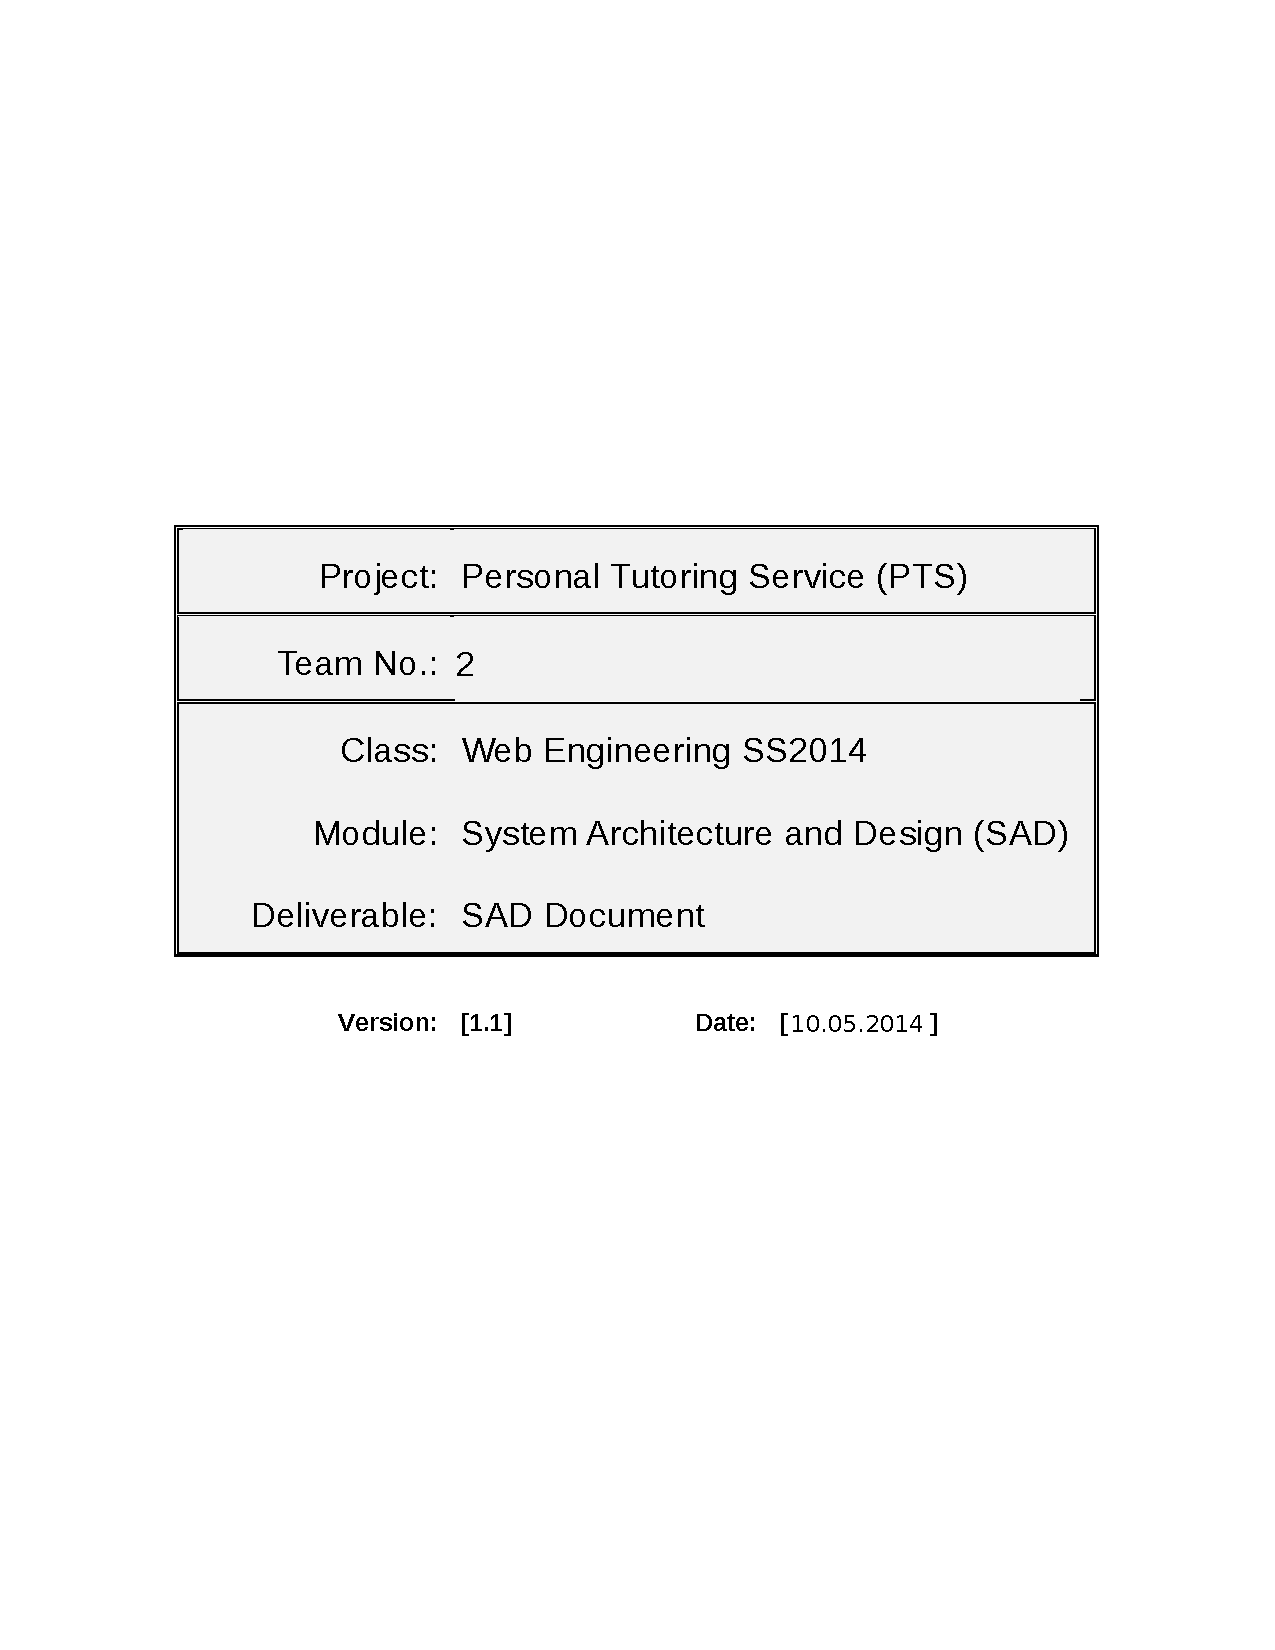
\includepdf{SAD_Titelseite.pdf}

\newpage
\begin{itemize}
\item[] \textbf{\large Beitragende:}\\
Sven Liebl\\
Matthias Goetz\\
Christian Dauerer\\
Maxmilian Schröter\\
Stefan Holz\\
Viet Nguyen\\
Daniel Tatzel\\
Nils Weiss\\
Florian Laufenböck\\
Alexander Strobl\\
Matthias Birnthaler\\
Tobias Schwindl
\end{itemize}

\bigskip

\begin{table}[!h]
 	\centering
	\begin{tabular}{|c|c|c|c||c|} 
	\hline
	\textbf{VersionsNr} &  \textbf{Datum} & \textbf{Auslöser} & \textbf{Veränderungsgrad} & \textbf{Beschreibung} \\
	\hline
	1.0 & 23.04.2014 & I-wer & Erster Entwurf & First Draft \\
	\hline
	\text{ } & \text{ } & \text{ } & \text{ } & \text{ } \\
	\hline
	\text{ } & \text{ } & \text{ } & \text{ } & \text{ } \\
	\hline
	\text{ } & \text{ } & \text{ } & \text{ } & \text{ } \\
	\hline
	\end{tabular}

\caption{Überarbeitungshistorie}
\end{table}

\newpage
\tableofcontents
% \listoftables

\section{Software Architecture}
%und alle anderen Diagramme!!
\subsection{Kontextdiagramm 1}
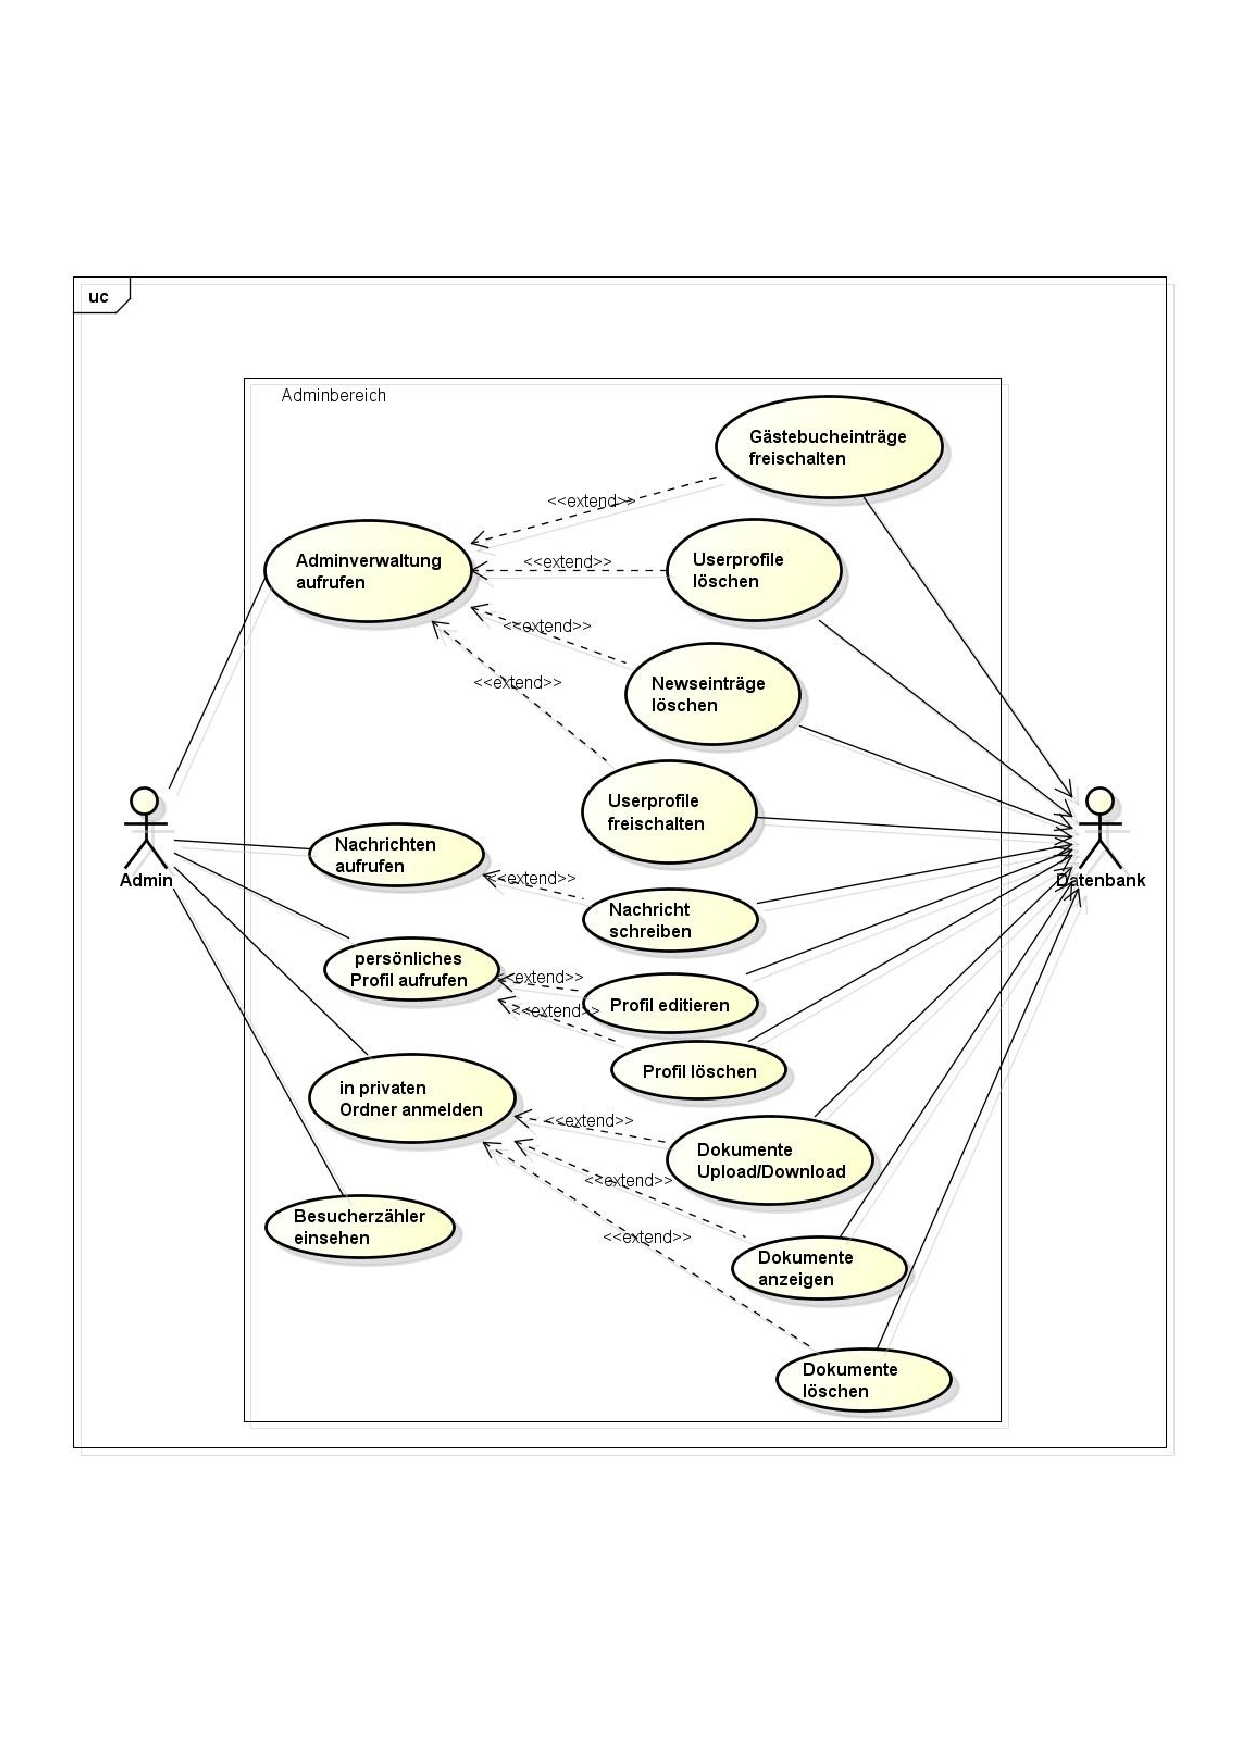
\includegraphics[width=0.9\textwidth]{./Source/UseCaseAdministrator_11.pdf}
\subsection{Kontextdiagramm 2}
\fbox{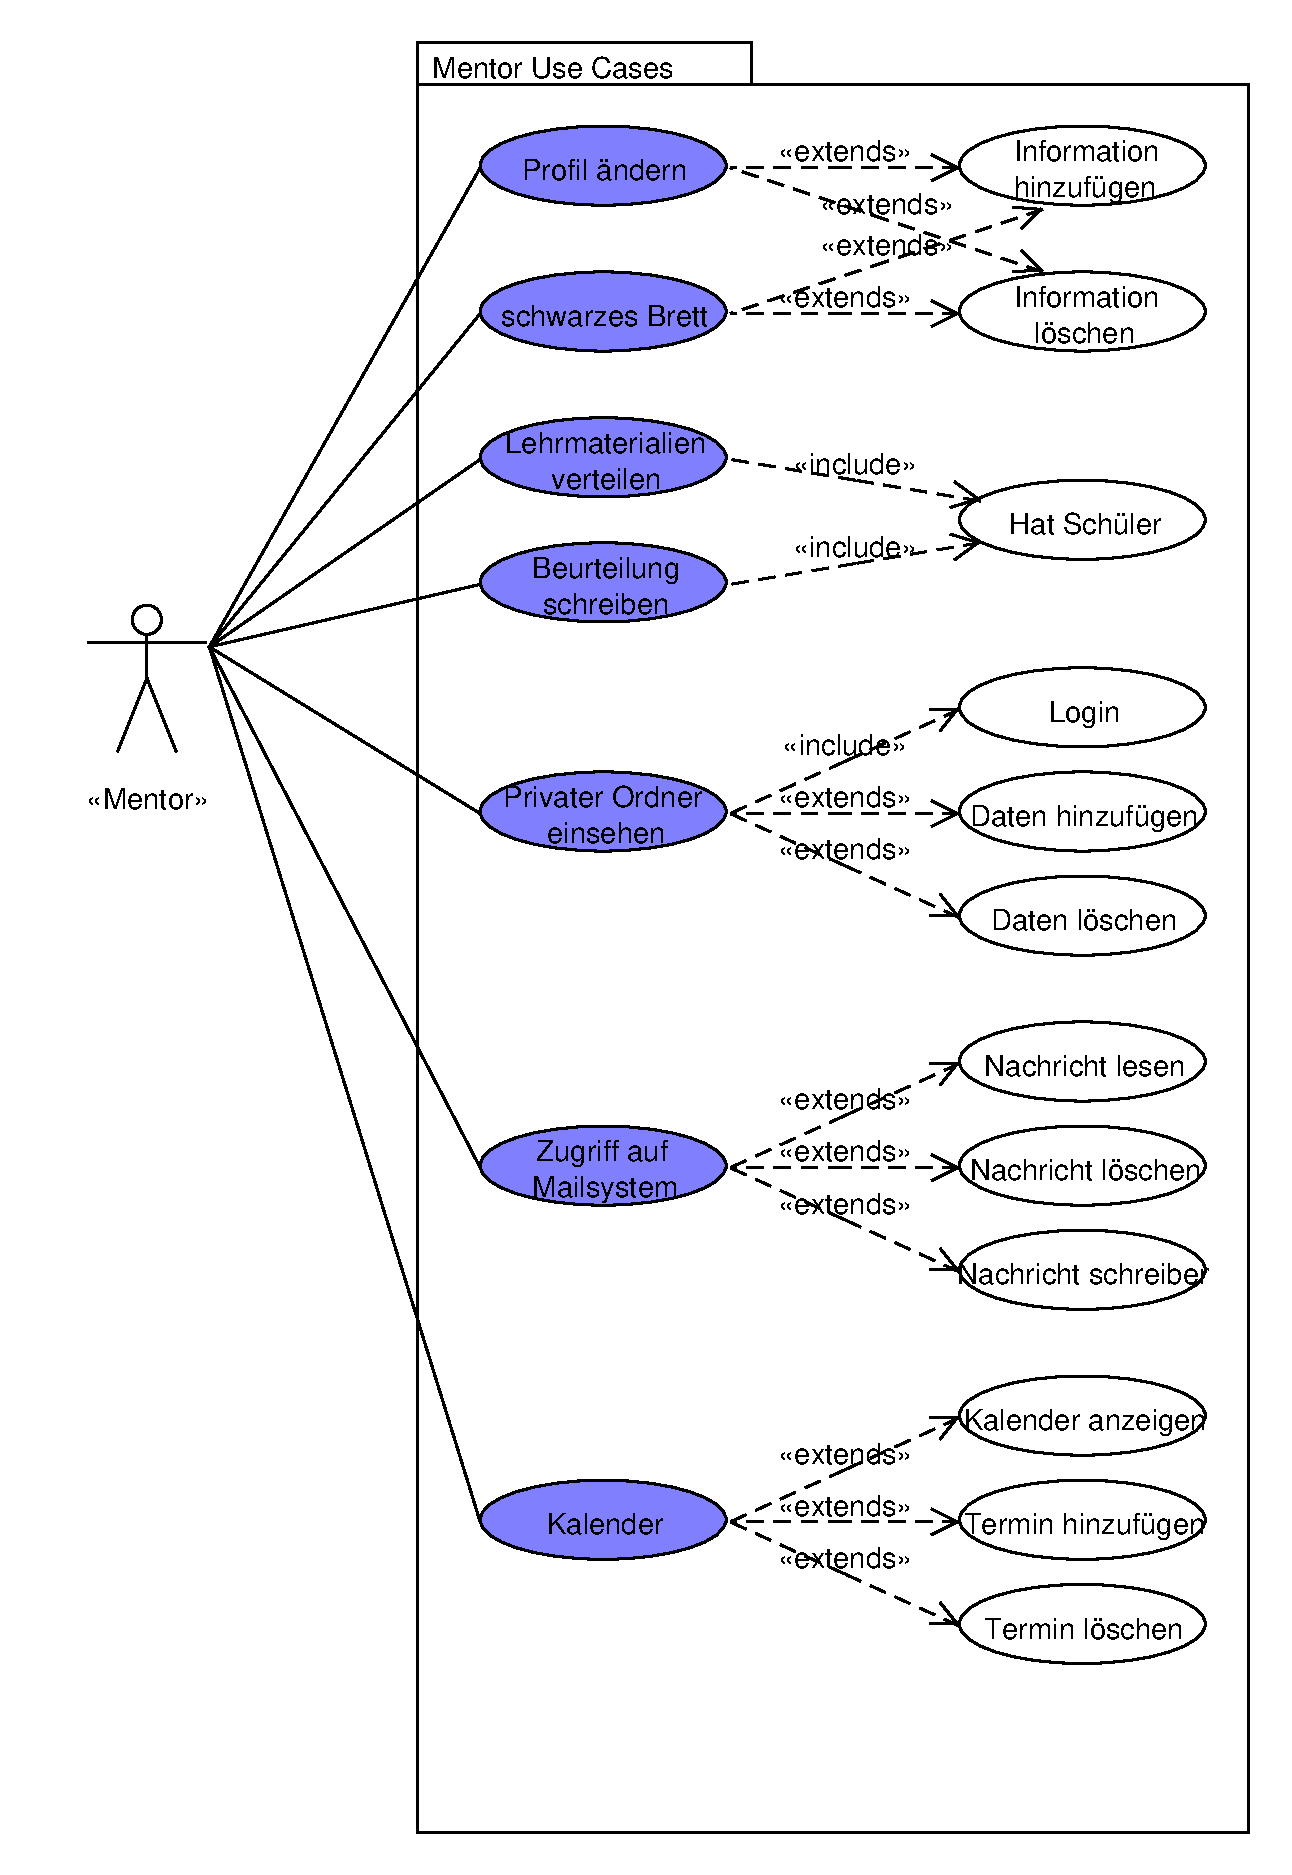
\includegraphics[width=0.9\textwidth]{./Source/UseCaseMentor_11.pdf}}

\section{Objectives} 

\subsection{Business Objectives}
Ziel der Webseite ist es Tutoren in der Nähe zu finden, und mit Ihnen in 
Verbindung zu treten. Durch die Möglichkeit ein persönliches Profil erstellen zu 
können, sollen Nutzer dauerhaft an unser Webangebot gebunden werden. 
Potentielle Nutzer sollen direkt an Hochschulen geworben werden. Auch 
Kooperationen mit Universitäten und Hochschulen sollen geschlossen werden.

Unser Webangebot soll kostenfrei sein. Finanziert werden soll das Angebot durch 
gezielte Werbung.

\subsection{System Objectives}
Das Webangebot Personal Tutoring Service soll als ``Template" aufgebaut werden. 
Somit soll es möglich sein, leicht andere Vermittlungsportale, wie z.B. eine 
Mitfahrzentrale aufzubauen. Somit sollen sich mit geringem Aufwand schnell neue 
Geschäftszweige erschließen lassen.

\section{Systems Requirement}

\subsection{F1: Öffentlicher Bereich}
\subsubsection*{F11: Startseite}
Matthias G. und Sven

Informiert den Besucher über das Auswahlkonzept bzw. $-$kriterien der Tutoren. Ebenfalls wird eine Karte mit den Standorten von Tutoren in Deutschland implementiert. Ein Teaser über das Motto und der Angebote der Website soll den Besucher ansprechen und so sein Interesse fördern. Durch die Anzeige von Top Gästebucheinträgen wird dem Gast das Gefühl der Vertrauenswürdigkeit und der Kompetenz übermittelt. 

Karte
Es wird eine Karte von Google-Maps eingebettet. Dies funktioniert mit Hilfe des bereitgestellten Iframes von Google.
Slideshow
Die Bilder der Slideshow werden mit HTML5 zur Verfügung gestellt. Mittels CSS3 werden die Bilder formatiert. JQuery sorgt für die Slideanimation. 
Video
Das Video wird mit HTML5 implementiert und ist dadurch ohne Flash abspielbar. Die Kontrollfunktionen werden ebenfalls mit HTML5 zur Verfügung gestellt.
Controls selbst erstellen

Top Gästebucheinträge
Nach dem Laden der Seite wird eine Javascript-Funktion ausgeführt, welche die Top-Gästebucheinträge über ein Json-Objekt erhält. Diese Einträge werden über JQuery eingeblendet und über CSS3 formatiert.

Profil bearbeiten
- HTML5 Formulare
- Formulare mit HTML5+ JS überprüfen (live)
- PHP Script ? Änderung


\subsubsection*{F12: Gästebuch}

Das Gästebuch ermöglicht den Nutzern eigene Kommentare abzugeben. Diese werden in einer SQL - Datenbank abgespeichert. Zusätzlich wird dazu der Autor abgespeichert und eine Variable, welche erfasst, ob ein Gästebuch eintragt bereits von einem Administrator autorisiert wurde, oder nicht. Mittels PHP, im speziellen mit dem PDO werden die Gästebucheinträge zum Frontend der Website weitergeleitet und dort angezeigt. Einträge, die sehr gute Bewertungen erhalten werden zur Werbung für die Website eingesetzt.

\subsubsection*{F13: Anzeige von verfügbaren Tutoren in der Nähe}

Stefan und Viet

Anhand einer Postleitzahlsuche ist im Voraus überprüfbar, ob Tutoren in der Nähe zu finden sind.

\subsubsection*{F14: Erweiterte Suchkriterien}

Backend

Beinhalten die Suche der gewünschten Schulart, Fach, Klasse, Preis und die maximale Fahrzeit zwischen Tutoren und Schülern. 

\subsubsection*{F15: Registrierungs- und Anmeldefenster}

Die Registrierung erfolgt über ein Formular, in der alle Daten, die unbedingt notwendig sind, ausgefüllt werden müssen.
Das OnlineFormular ist im \underline{HTML5} standard geschrieben, um gleich Validierungen der Eingaben durchführen zu können, 
ohne die Informationen erst zum Server schicken zu müssen.

Eingaben, die eindeutig sein sollen(wie z.B. der Benutzername) werden während der Eingabe mittels \underline{AJAX,JAVASCRIPT} 
zum Server geschickt und dort überprüft, sodass der Benutzer sofort erfährt(ohne auf einen Button klicken zu müssen), ob dieser Benutzername schon vergeben ist. Wenn alle Daten eingegeben wurden, die Validierungen erfolgreich waren, klickt der Benutzer auf einen Button und schickt die Daten damit zum Server. Dort werden die Daten mittels \underline{PHP} zur \underline{Datenbank} geschickt, um dort gespeichert zu werden.

\bigskip

Ist ein Nutzer registriert, so kann er sich über die Login-Maske, die auf jeder Seite eingebunden ist, registrieren. Hierfür wird eine Datenbank Abfrage mittels PHP und SQL über PDO generiert um die Identität des Nutzers zu prüfen. Bei erfolgreicher Authentifizierung der Benutzerdaten werden mehrere Sesseion-Variablen, die angeben, dass der Benutzer angemeldet ist und um welchen Benutzer es sich handelt, initialisiert um immer entsprechende Informationen über den Benutzer zu haben.

\subsubsection*{F16: About us (Impressum)}

Alex

Das Impressum enthält folgende Informationen: Firma, Straße, Postleitzahl, Ort, Telefonnummer, E-Mailadresse, Internetadresse, Vertretungsberechtigter, \\ Geschäftsführer, Inhaltlich Verantwortlicher und Haftungshinweis. 

\subsubsection*{F17: Preismodell/Zahlungsinfos}

Statisch, irgendwer

Informiert vorab über die Zahlungshinweise und Preise, um Irrtümer zu vermeiden.

\subsubsection*{F18: Auswahl der Sprache}

Die Auswahl der Sprache erfolgt über eine \underline{Serverseitige} \underline{Sessionvariable}, mit Hilfe derer 
die Serverseitig eingesetzte Skriptsprache \underline{PHP} sich über den gesamten Verlauf der Interaktion mit dem User "merken" kann,
welche Sprache der User benutzen will. Alternativ kann ein zusätzliches \underline{Feld} in der \underline{Datenbank} für die 
Sprache reserviert werden, womit bei jedem neuen Einloggen des Benutzers die Sprache automatisch ausgewählt wird. Sollte der Benutzer
die Sprache dann doch einmal ändern, wird diese Änderung unverzüglich in die \underline{Datenbank} geschrieben.
Umgesetzt wird das erstellen des Formulars so umgesetzt:
\begin{itemize}
 \item Für jeden Teil der Seite gibt es eine Vorlage in den Sprachen(z.B. Impressum)
 \item \underline{PHP} wählt dann zur Laufzeit aus, welche Elemente der Seite in der Sprache geladen werden muss
 \item und fügt alle Elemente mit Hilfe einer leeren "Dummy"Datei zu einer, korrekten, \underline{HTML5} Datei zusammen
 \item welche dann an den Client geschickt wird.
\end{itemize}

\subsubsection*{F19: Support und Kontaktdaten}

Alex

Persönliche Hilfen oder Anfragen, sind an den Support zu stellen. Erreichbar ist der Support per E-Mail. 


\subsection{F2: Administrator}
\subsubsection*{F21: Anmelden}

Backend

Der Administrator meldet sich mit einem Nutzernamen und einem Passwort an, um den privaten Adminbereich betreten zu können.

\subsubsection*{F22: Persönliche Einstellungen}

Matthias G und Sven

Wie jeder Nutzer verfügt der Administrator über ein persönliches Profil welches Vorname, Nachname, Geburtsdatum, Profilbild, Straße, Hausnummer, Wohnort, E-Mail, Telefon und Handynummer enthält. Die Bearbeitung und Löschung dieser Informationen ist über entsprechende Masken und Formularen zu er-möglichen.

\subsubsection*{F23: Bearbeiten von Kundenkonten$^1$ und Kundeninformationen$^2$}

Ist ein Nutzer als Administrator eingeloggt, hat dieser die Möglichkeit sich eine Übersicht
aller Kundenkonten anzeigen zu lassen. Diese Informationen werden in Form einer Tabelle auf 
einer separaten Seite angezeigt. Beim Aufruf der Seite werden alle notwendigen Informationen 
über Ajax aus der Datenbank geladen und über JSON an den Browser des Admins geliefert. Um
bei einer großen Datenbank die Wartezeit gering zu halten, werden die Daten nur teilweise
aus der Datenbank geladen. So ist es beispielsweise nicht sinnvoll mehr wie 20 Datensätze 
gleichzeitig zu laden, da in der Regel nicht mehr angezeigt werden kann.

Durch eine Tabellen-PlugIn für jQuery werden die Rohdaten übersichtlich dargestellt.
Die Tabelle soll außerdem die Möglichkeit bieten die Datensätze nach Spalten zu sortieren.

Änderungen der Daten werden ebenfalls über jQuery an die Datenbank übergeben, wenn der Administrator
einen "Speichern" Knopf drückt.

Die Validierung der Daten wird über HTML5 und gegebenenfalls mit einer PHP-Funktion durchgeführt.

\subsubsection*{F24: Zugriff auf Nachrichtensystem}

In der Datenbank befinden sich eine große Tabelle in der alle Nachrichten als Rohdaten abgelegt werden.
Jeder Datensatz hat die Felder: Absender, Empfänger, Datum, Zeit, Nachricht, gelesen.
Über SQL-Abfragen werden die jeweiligen Nachrichten aus der Datenbank geladen und über JSON an ein
jQuery-Script übergeben. Möchte ein Nutzer Beispielsweise alle gesendeten Nachrichten einsehen, wird
der aktuell angemeldete Nutzername in die "WHERE"-Klausel der Datenbankabfrage eingefügt, um so nur 
die relevanten Nachrichten abzufragen.

Zum Abrufen der Nachrichten wird dem angemeldeten Nutzer eine spezielle Webseite zur Verfügung gestellt,
auf welcher er Nachrichten abrufen und erstellen kann. Die Anzeige wird in Form einer Tabelle über
ein jQuery-Plugin erstellt. 

Zum Versenden von Nachrichten muss ein Nutzer den Benutzernamen eines Empfängers in ein Textfeld eingeben.
Bevor eine Nachricht abgesendet werden kann, erfolgt eine Validierung des Benutzernamens des Empfängers.
Diese Validierung wird durch ein Javascript vorgenommen. 
Für das Eingabefeld des Empfängers ist es denkbar eine Autovervollständigung über Ajax zur Verfügung zu stellen. 

\subsubsection*{F25: Freischaltung von Gästebucheinträge}

Der Administrator ruft das Gästebuch auf und sieht alle nicht autorisierten Einträge. Diese kann er dann autorisieren. Dann werden diese in der Datenbank aktualisiert.

\subsubsection*{F26: Abmelden}

Jeder angemeldete Nutzer kann sich auch wieder abmelden, dies geschieht durch löschen einer Session-Variable, die bei der erfolgreichen Anmeldung gesetzt wurde. Das löschen der Variable hat keinen Einfluss auf die restlichen Inhalte der Session.

\subsubsection*{F27: Besucherzähler}

Für jeden Besucher der Seite wird eine PHP Session in Form eines Cookies, der drei Stunden aktiv ist, initialisiert. Bei jedem Aufruf wird geprüft, ob eine Session-Variable, die zur Erkennung benutzt wird, gesetzt ist. Falls diese nicht gesetzt ist, dann wird der Besucherzähler um eins erhöht. Ist die Variable jedoch gesetzt, dann wurde der Besucher schon gezählt und es wird nichts unternommen.

\bigskip

$^1$ Kundenkonten: Tutorenkonten und Schülerkonten\\
$^2$ Kundeninformationen: Persönliche Informationen der Kundenkonten

\subsection{F3: Schüler}
Jeder Besucher hat die Möglichkeit ein Profil anzulegen und sich mit den erhaltenen Zugangsdaten einzuloggen.
Dadurch erhält er Zugriff auf seinen Privaten Bereich, in dem er seine bei der Registrierung hinterlegten persönlichen Daten ändern kann.
Die persönlichen Daten setzen sich aus Vorname, Nachname, Alter, Anschrift, Schultyp, Jahrgangsstufe, Passwort Kontaktdaten und Profilbild zusammen. 
Es besteht die Option seinen Account zu löschen.

\subsubsection*{F31: Detaillierte Suche}

Die Suche wird mittels einer View realisiert. Diese View enthält alles notwendigen Informationen, die es dem User ermöglichen das gewünschte Suchergebnis zu finden, 
 - Benutzername
 - Wohnort
 - Umkreis
 - Stundenlohn
 - Bewertung
 - Fächer
 - Stufen
Die View wird verwendet um in den normalen Tabellen keine Redundanzen zu haben. 

\subsubsection*{F32: Tutorprofil/Tutorbewertung}

Matthias G und Sven

Der registrierte Anwender ist berechtigt das Profil des Tutors einzusehen, das für den Anwender folgende Informationen bereit hält:

\begin{itemize}
	\item Geschlecht
	\item Stundenlöhne 
	\item Verfügbarkeiten 
	\item Fächer / Jahrgangsstufen 
	\item Verfügbare Orte / Regionen - Eintrag auf Karte
	\item Profilbild
	\item Kontaktdaten
	\item Lehrerbewertung
\end{itemize}
	
Er ist in der Lage das Schwarze Brett des Tutors einzusehen.

\subsection*{F33: Zahlungsinformationen}

Der Schüler zahlt mit Kreditkarte. Dazu gibt er seine Kreditkarteninformationen in ein HTML5 Formular u. a. Name, Vorname, Benutzername, Kreditkartennummer, Ablaufdatum der Karte, die Prüfziffer und den zu zahlenden Betrag. Diese werden auf Richtigkeit der Informationen geprüft (HTML5 Formular) und dann für die weitere Verwendung in der MySQL Datenbank gespeichert. 

\subsection{F4: Lehrer / Mentor}
\subsubsection*{F41 Profil einstellen}

Matthias G und Sven

Der Tutor kann ein Profil erstellen, um sich kurz vorzustellen und Werbung in eigener Sache machen zu können. Schüler können ihn bewerten (z.B. Verbesserung der Note).

Das Profil soll beinhalten / anbieten:
\begin{itemize}
	\item Geschlecht
	\item Stundenlöhne verlangen
	\item Verfügbarkeiten angeben
	\item Fächer / Jahrgangsstufen einstellen
	\item Verfügbare Orte / Regionen anbieten - Eintrag auf Karte
	\item Zahlungsdaten zur Verfügung stellen
	\item Sieht in einer Übersicht seine Schüler und einen Kalender mit den nächsten Terminen
	\item Rechnungen / Zahlungserinnerungen verschicken
	\item Profilbild
	\item Kontaktdaten
	\item Lehrerbewertung / Gästebuch
\end{itemize}

% \subsubsection*{F42 Lehrmaterialien online stellen und verteilen}
% 
% Jeder Schüler muss sich in Online-Kurse eintragen, bei welchem Tutor er welches Fach belegt. Der Tutor kann über einen Upload-Bereich(jquery bietet diese Möglichkeit) Dateien zum Server laden, dort werden diese in der \underline{Datenbank} gespeichert.
% Der Schüler kann sich dann die Formulare über den Browser wieder herunterladen
% 
% \subsubsection*{F43 Beurteilungen schreiben}
% 
% Stefan und Viet
% 
% Der Schüler kann Feedback für seine abgegeben Aufgaben / Leistungen erhalten

\subsubsection*{F42 Schwarzes Brett}

Stefan und Viet

Der Mentor kann allgemeine Informationen hinzufügen z.B. bei Krankheit


\section{Annahmen und Beschränkungen}
\subsection{Annahmen}

\subsection{Beschränkungen}

\subsubsection*{Leistung}

Einer der wichtigesten Dinge, auf die zu achten ist, ist die Kommunikation zwischen \underline{javascript} und \underline{PHP} 
über \underline{AJAX}. Wenn man mit Hilfe von javascripts Daten dynamisch über PHP bzw. PDO aus einer Datenbank laden will, sollte man
sehr genau auf die Performance dieses Prozesses achten. Wenn man also *.php Skripte ansteuert, sollte man in diesen darauf achten, dass
das Skript an sich sehr performant ist(z.B. nicht viele, große Klassenobjekte generieren, Operationen durchführen die sehr lange brauchen,
wie z.B. aufwendige Hash-Operationen), da sonst die Datengenerierung im PHP-Skript sehr lange dauert und dies dazu führt, dass 
es relativ lange dauert, bis aktualisierte Informationen auf dem Bildschirm des End-Users angezeigt werden.

Um diesem Umstand gerecht zu werden, sollen die Files so angelegt werden, dass pro File möglichst wenig Funktionen enthalten sind.
Damit soll ein möglichst hoher Grad an Unabhängigkeit von anderen Funktionen erreicht werden, sodass in jedem *.php File nur die 
für die darin enthaltenen Funktionen benötigten Komponenten ausgeführt werden müssen.

\subsubsection*{PHP Funktionen aus Javascript}

Da man mit Hilfe javascript nur einzelne *.php-Skripte ansprechen kann und nicht einzelne Funktionen aus php wird es für die meisten javascript-Funktionen eine *.php-Datei geben, die dann die Dinge ausführt, die Serverseitig gemacht werden sollen. Damit kann man auch mehrere Serverseitige Methoden auf ein Mal abarbeiten.


\subsubsection*{Datenbank}

\begin{enumerate}
 \item Durch das Einsetzen einer MySQL Datenbank sind wir durch das Relationale Design in der Optimalen Aufteilung, wie man es bei einem NoSQL System umsetzen würde um bessere Reaktionszeiten zu erhalten, eingeschränkt.
 \item Durch den Einsatz eines einzigen Entitätstyp für den Besucherzähler ist die maximale Anzahl an neuen Nutzer, die gleichzeitig auf die Seite zugreifen, die gezählt werden können begrenzt.
 \item Benutzernamen dürfen maximal eine Länge von 20 Zeichen haben um unnötigen Speicherplatz zu vermeiden.
 \item Um so wenig NULL Werte wie möglich zu bekommen, ist darauf zu achten, dass
\end{enumerate}

%\section{Glossar}

\end{document}



